%% 
%% 報告書の LaTeX サンプル
%%	(version 4.4) 2015/07/14
%%

%\documentclass[bigbox]{jarticle}
\documentclass{jarticle}[11pt]
%\documentstyle[bigbox,fancybox]{jarticle}

% コマンドの定義
%
% コメントアウト用のコマンド
%   複数行にまたがる記述をまとめてコメントアウトする際に利用できる
%   \COMMENT{ .... } で .... の部分をコメントアウト
\newcommand{\COMMENT}[1]{}

% 以下は,表(srmmary.tex)で使用しているコマンド
\newcommand{\lw}[1]{\smash{\lower2.ex\hbox{#1}}}

% 図を参照するためのマクロ
\newcommand{\figref}[1]{\makebox{図~\ref{#1}}}

% 表を参照するためのマクロ
\newcommand{\tabref}[1]{\makebox{表~\ref{#1}}}

%% 使用しているパッケージ等があれば,宣言しておく
\usepackage{ascmac}

\usepackage{graphicx}

% 以下のパラメータは,見易いように適宜調整する.
\textwidth=15cm
\oddsidemargin=-.2cm
\evensidemargin=-.2cm
%\topmargin=-1cm

%% 報告書のタイトル,提出者,提出日等
%% これらのための専用の表紙を設ける必要はない.

%% 以下のタイトルは適切に変更すること
%% レポートに (version 4.4) などの記述不要なので削除のこと
\title{{\normalsize 情報工学実験(ハードウェア実験)報告書}\\
PARTHENONによる32ビットマイクロプロセッサの作成 }


%% 自分の学生番号と名前に変更すること.
\author{ 
  学生番号: 09425566 \\
  提出者: 佐藤 佑太
}

%% 提出日を記載する.
\date{
  提出日: 2015年 7月27日 \\
  締切日: 2015年 7月27日
}

\begin{document}
\maketitle

%%        1         2         3
%%2345678901234567890123456789012345678
%% (参考)
%% Emacs等のエディタでは通常,横に全角文字を40文字(半角で80文字)表示
%% できるため,このサンプルファイルのテキストは各行を34〜38文字程度に収まる
%% ように適宜改行を入れている.
%% テキスト中に改行をいれていても,LaTeXで整形後にその改行は出力されない.
%% 適切に改行をいれておくほうが,テキストの編集をしやすいため,こうしている.
%% 改行の箇所は,文章の編集しやすさを考慮して,可能な限り句読点の箇所や
%% 文章,文節の区切りでいれている.
%% Emacsでは 
%%   C-a ....... 行頭にカーソルを移動
%%   C-k C-k ... カーソルから行末までをコピーして削除(カット)
%%   C-y ....... カーソル位置にコピーしたテキストをはき出す(ヤンク).
%% で編集できるため,文章の区切りのよい箇所で改行を入れて別の行に記述して
%% おくほうが編集を容易に行うことができる.
%% 
%% 

\begin{abstract}
% (ここに報告書の概要を簡潔にまとめる.
% 本文中にある文章をピックアップしつなげてまとめることで作成する.
% 特に「おわりに」にある文章が活用できる場合が多い.)

本稿では,情報工学実験(ハードウェア実験)において作成した、
32ビットマイクロプロセッサについてまとめる。
\end{abstract}


\section{はじめに}

% 報告書の最初の節(ここでは「{\gt はじめに}」というタイトルとしている)では,
% 実験の背景と目的,および,本報告書の構成について述べる.
% 報告書の構成は,各自の判断で分かりやすい構成にすればよい.
% このサンプルでは,{\bf 1} 〜 {\bf 4} 節の構成をとっているが,
% 報告事項によって適宜変更する.
% 各節では小節(subsection)を設けるなどして,わかり易い構成をとって欲しい.
% %% パラグラフを変える場合,次の行のように空行を1行以上入れればよい.
% 
% 以下に,かなり省略してはいるが,「{\gt はじめに}」の記述例を示す.
% 節(section)や小節(subsection)等の参照には,\verb|\ref{ラベル名}|
% といった記述を用いる.
% ラベルの定義は,本ドキュメントのソースの見ればわかるだろう.

% パラグラフの冒頭で段下げをしたくない場合,下のように \noindent と書く
\noindent

本実験の目的は、ハードウェア記述言語とCADツールを利用したマイクロプロセッサの設計を通して、
論理回路、コンピュータアーキテクチャ、およびコンピュータシステムに関する理解を
深めることである。

本報告書では,ハードウェア記述言語とCADツールを用いた論理回路の設計と、
32ビットマイクロプロセッサの設計について報告する.

% 次の行は,参考文献の引用例.〈文献のラベル〉を \cite{} で括る.

%情報工学実験テキスト \cite{bib:実験テキスト} の第1章から第3章の
%.... .... .... .... .... を報告する.

本報告書の構成は次のとおりである.
まず 
{\bf \ref{sec:設計したプロセッサの概要}} にて本実験で設計したプロセッサの概要
について述べる.

{\bf \ref{sec:実施状況の報告}} にて本実験における実施内容の状況報告を行う。

{\bf \ref{sec:プログラミング課題に関する報告}}では,アセンブリによって作成したプログラムの
作成に関しての報告を行う。

{\bf \ref{sec:プロセッサ設計課題に関する報告}}では,作成したプロセッサの設計に関して
報告を行う。

{\bf \ref{sec:追加課題や発展課題に関する報告}}では,発展課題で取り組んだ課題について報告する。

{\bf \ref{sec:検討・考察}}では,諸事項について検討を行い、それについての考察を記述する。

{\bf \ref{sec:工夫した点や特に力を注いだ点}}では,設計の際に工夫した点や特に注力した点について報告する。

{\bf \ref{sec:本実験を実施して得られたこと}}では,本実験を通して、
どこれまでから一層理解が深まった部分などについて記述する。

{\bf \ref{sec:進捗状況報告}}では,本実験の進捗状況報告ファイルを掲載する。

{\bf \ref{sec:作成した設計記述、プログラム等のリポジトリ名、ファイル名の一覧}}では,
本実験で作成したアセンブリ言語プログラム、設計したSFL記述、テスト用スクリプト、テスト結果、
論理合成時の出力等のファイルの一覧を掲載する。

最後に {\bf \ref{sec:おわりに}} で,本報告のまとめと今後の課題を述べる。




%%%%%%%%%%%%%%%%%
%   SECTION 2   %
%%%%%%%%%%%%%%%%%

\section{設計したプロセッサの概要}
\label{sec:設計したプロセッサの概要}

ここでは,設計したプロセッサの概要について述べる.

本実験で設計したプロセッサは32ビットRISCマイクロプロセッサとなっており、
コプロセッサやキャッシュメモリは実装されていない。

アセンブリ言語はMIPSのものとほぼ同様のものとなっている。

%また、各プロセッサの構造は
%
%\begin{enumerate}
%\item p32m1
%\end{enumerate}
%p32m1...マルチサイクルバージョン
%1命令を5サイクル



\subsection{サポートする命令セット}

まず、本実験でサポートする命令セットを以下の表に示す。

\begin{table*}[htb] % table* だと1カラム配置(横長)の表になる
\caption{サポートする命令一覧}
\label{サポートする命令一覧}
\begin{center}
% 以下のサンプルは,p32においてデフォルトでサポートする命令一覧となっている.
% これをベースに命令を削除,あるいは追加するとよい
% もし,以下のサンプルに記載されていない命令のサポートを行う場合,ボールド体
% にて書いておく(例: {\bf add})
\begin{tabular}{c|p{6cm}|p{4cm}}
\hline \hline
命令種別 & 
\multicolumn{1}{c}{サポートする命令} &
\multicolumn{1}{|c}{サポートしない命令} 
\\ \hline

算術論理演算 &
% サポートする命令
add, addu, addi, addiu, sub, subu, 
and, andi, or, ori, xor, xori, nor &
% サポートしない命令(以下に書く)
mult, multu, div, divu
\\

比較 &
% サポートする命令
slt, sltu, slti, sltiu &
% サポートしない命令(以下に書く)
\\

シフト &
% サポートする命令
sll, srl, sra, sllv, srlv, srav &
% サポートしない命令(以下に書く)
\\

ロートストア &
% サポートする命令
lw, sw, lb, sb &
% サポートしない命令(以下に書く)
\\

分岐 & 
% サポートする命令
beq, bne &
% サポートしない命令(以下に書く)
\\

ジャンプ &
% サポートする命令
j, jr, jal, jalr &
% サポートしない命令(以下に書く)
\\

データ転送 &
% サポートする命令
lui, mfhi, mflo &
% サポートしない命令(以下に書く)
\\

例外,システムコール &
% サポートする命令
syscall &
% サポートしない命令(以下に書く)
\\

\hline
\end{tabular}
\end{center}
\end{table*}


今回は掛け算、割り算の命令については時間が足りなかったため実装しないこととした。


% 内部構造の概略 

% 処理方式の概略



%%%%%%%%%%%%%%%%%
%   SECTION 3   %
%%%%%%%%%%%%%%%%%

\section{実施状況の報告}
\label{sec:実施状況の報告}

ここでは,取り組んだ課題の実施状況について報告する。

\subsection{報告内容に関する事項}
私たちの班では、役割分担をせずにそれぞれがプログラムの作成を行った。
そのため、各プログラムにおける個人の役割は100中全員がすべて100であると
考えたため、表からは省略している。

課題の実施内容は、以下の表のようになっている。

\begin{table*}[htb] % table* だと1カラム配置(横長)の表になる
\caption{実施状況}
\label{実施状況}
\begin{center}
% 以下のサンプルは,p32においてデフォルトでサポートする命令一覧となっている.
% これをベースに命令を削除,あるいは追加するとよい
% もし,以下のサンプルに記載されていない命令のサポートを行う場合,ボールド体
% にて書いておく(例: {\bf add})
\begin{tabular}{c|p{6cm}|p{4cm}}
\hline \hline
設計課題番号 & 
\multicolumn{1}{c}{内容} &
\multicolumn{1}{|c}{実施} 
\\ \hline

D-1 &
32ビット加算器add32の設計 &
実施済み 
\\

D-2-1 &
カウンタの設計 &
実施済み 
\\

D-2-2 &
カウンタの設計 &
未実施
\\

D-2-3 &
カウンタの設計 &
未実施
\\

D-3 &
32ビットALUの設計 &
実施済み
\\

D-4 &
32ビットシフタの設計 &
実施済み
\\

E-1 &
32ビットCarry Lookahead Adderの設計 &
未実施
\\

E-2 &
32ビット整数乗算器の設計 &
未実施
\\

E-3 &
32ビット除算器の設計 &
未実施
\\

5-1 &
5ビット比較器 &
実施済み
\\

5-2 &
レジスタファイル &
実施済み
\\

5-3 &
メモリユニット &
実施済み
\\

6-1 &
p32プロセッサコア(マルチサイクル) &
実施済み
\\

E6-1 &
p32プロセッサコアの改良 &
未実施
\\

E6-2 &
乗算機能の実装 &
未実施
\\

7-1 &
p32プロセッサコア(マルチサイクルv2) &
実施済み
\\

E7-1 &
p32プロセッサコアの改良 &
未実施
\\

E7-2 &
乗算機能の実装(2) &
未実施
\\

8-1 &
p32プロセッサコア(パイプライン) &
実施済み
\\

E8-1 &
p32プロセッサコアの改良 &
未実施
\\

\hline
\end{tabular}
\end{center}
\end{table*}




\newpage

%%%%%%%%%%%%%%%%%
%   SECTION 4   %
%%%%%%%%%%%%%%%%%

\section{プログラミング課題に関する報告}
\label{sec:プログラミング課題に関する報告}

ここでは,アセンブリで実装したプログラミング課題3に関しての報告を行う。

プログラミング課題3では、整数をソートするプログラムの作成を行った。
当初はクイックソートでソートプログラムを作成したいと考えていたが、
実装のしやすさからバブルソートによるソートプログラムを作成した。


%TODO
%%%%%%%%%%%%%%%%%
%   SECTION 5   %
%%%%%%%%%%%%%%%%%

\section{プロセッサ設計課題に関する報告}
\label{sec:プロセッサ設計課題に関する報告}

ここでは,プロセッサ設計課題に関する報告を行う。

\subsection{設計課題6-1}

設計課題6-1では、マイクロプロセッサp32のコアモジュールとなるp32m1,p32m2,p32p1の設計を行った。

各サブモジュールを論理合成した結果、以下の表のような数値が得られた。


\begin{table}[htb]

\caption{論理合成で得られた諸量のまとめ}
\label{tab:論理合成で得られた諸量のまとめ}
\begin{center}
% 表が大きいので,tiny サイズのフォントを利用
{\tiny
\begin{tabular}{l|cccccc}
\hline
\hline
\lw{モジュール}
& 最大遅延 & 最大動作周波数 & \lw{ゲート数} & 実装面積 & 消費電力 &
最大動作周波数で \\
& (ns) & (MHz) & & (1000$\mu$m$^2$) & ($\mu$W/MHz) & 動作時の消費電力 \\
\hline
%4ビット加算器     & & & & & & \\
32ビット加算器     &33.1 &30.21& 95& 25.18& 224.0& 6.77 \\
%4ビット桁上げ先見加算器 & & & & & & \\
%8ビット桁上げ先見加算器 & & & & & & \\
%16ビット桁上げ先見加算器 & & & & & & \\
%4ビットALU    & & & & & & \\
%16ビットALU    & & & & & & \\
32ビットALU    & 125.3& 30.21& 95& 25.18& 224.0& 6.77\\
%8ビットシフタ     & & & & & & \\
%16ビットシフタ     & & & & & & \\
32ビットシフタ     & 26.6& 27.32& 2488& 267.91& 2519.8& 68.85\\
5ビット比較器     & 24.0& 41.67& 27& 6.26& 67.1& 2.80\\
レジスタファイル     & 31.6& 31.65& 17871& 4888.41& 34645.4& 1096.37\\
%メモリユニット     & & & & & & \\
p32プロセッサコア(マルチサイクル)   & 125.0& 8.00& 30512& 8240.88& 57859.9& 462.88\\
p32プロセッサコア(マルチサイクルv2)   & 124.5& 8.03& 30994& 8357.85& 58670.4& 471.25\\
p32プロセッサコア(パイプライン)   & 230.9& 4.33& 31991& 8597.80& 60738.8& 263.05\\
%10進カウンタ  & & & & & & \\
%4ビットアップダウンカウンタ   & & & & & & \\
\hline
\end{tabular}
}
\end{center}
\end{table}


% TODO
%%%%%%%%%%%%%%%%%
%   SECTION 6   %
%%%%%%%%%%%%%%%%%

\section{追加課題や発展課題に関する報告}
\label{sec:追加課題や発展課題に関する報告}


今回は追加課題や発展課題に取り組む時間を確保することができず、実装することができなかった。


% TODO
%%%%%%%%%%%%%%%%%
%   SECTION 7   %
%%%%%%%%%%%%%%%%%

\section{検討・考察}
\label{sec:検討・考察}

全体的にプロセッサ自体を仕上げることのみにしか時間を割くことができず、
細部でよりよいパフォーマンスをだすための工夫などを施すことができなかった。



% TODO
%%%%%%%%%%%%%%%%%
%   SECTION 8   %
%%%%%%%%%%%%%%%%%

\section{工夫した点や特に力を注いだ点}
\label{sec:工夫した点や特に力を注いだ点}

プロセッサに使われているモジュールを逐一しっかりと挙動をりかいしながら
プロセッサを設計することをこころがけた。そうすることでよりプロセッサの挙動を
理解しながら設計し、そこから性能をあげるような実装もできるのではないかと考えたが、
今回そこまでの時間をとることができなかった。


% TODO
%%%%%%%%%%%%%%%%%
%   SECTION 9   %
%%%%%%%%%%%%%%%%%

\section{本実験を実施して得られたこと}
\label{sec:本実験を実施して得られたこと}

自分が使っているコンピュータが、根本ではどのように作用しているのか
理解することができた。


%%%%%%%%%%%%%%%%%
%   SECTION 10  %
%%%%%%%%%%%%%%%%%

\section{進捗状況報告}
\label{sec:進捗状況報告}

この章では、設計課題の進捗状況を報告する。

設計内容の進捗は以下に掲載する。

\begin{verbatim}
(設計課題進捗状況)

グループ: B-10
学生番号: 09425566
氏  名: 佐藤佑太
最終更新: 2015-06-23(火) 18:00

       | (2)  | | (3)  | | (4)  | | (5)  | | (6)  | | (7)  | | (8)  | | (9)  | 
       | 5/26 | | 6/2  | | 6/9  | | 6/16 | | 6/23 | | 6/30 | | 7/7  | | 7/14 |
課題   | 3 4 5| | 3 4 5| | 3 4 5| | 3 4 5| | 3 4 5| | 3 4 5| | 3 4 5| | 3 4 5|
-------+------+-+------+-+------+-+------+-+------+-+------+-+------+-+------+
(D-1)  |  <+T                                                               S>
(D-2-1)|    <+ttttttttttttT>                                             
(D-2-2)|  
(D-2-3)|  
(D-3)  |                    <+tttT                                          S> 
(D-4)  |                           <++ttT                                   S>
(E-1)  |
(E-2)  |
(E-2)  |
(5-1)  |                                  <+T                                S>
(5-2)  |                                     <+T                             S>
(5-3)  |                                        <++T>                    
(6-1)  |                                             <++++tttttttttT         S>
(E6-1) |
(E6-2) |
(7-1)  |                                                   <+++++ttttttT     S>
(E7-1) |
(E7-2) |
(8-1)  |                                                              <+tttT S>
(E8-1) |
-------+------+-+------+-+------+-+------+-+------+-+------+-+------+-+------+

(シンボルとその説明)
  < ... 着手
  + ... 実施(コーディング)
  t ... Secondsシミュレーション,デバッグ
  T ... Secondsシミュレーション,デバッグ 完了
  v ... Verilog HDL シミュレーション,デバッグ
  V ... Verilog HDL シミュレーション,デバッグ 完了
  S ... 論理合成  
  > ... 完成
  * ... 実施(改良等)
  . ... その他
※ シンボルは半角文字で書くこと(全角文字は使わない)

(基本モジュールの設計)
(D-1)  【設計課題2-1】〜【設計課題4-1】	32ビット加算器add32の設計
(D-2-1)【設計課題2-2】〜【設計課題4-2】	カウンタの設計(_-2-1)
(D-2-2)【設計課題2-2】〜【設計課題4-2】	カウンタの設計(_-2-2)
(D-2-3)【設計課題2-2】〜【設計課題4-2】 カウンタの設計(_-2-3)
(D-3) 【設計課題2-3】〜【設計課題4-3】  32ビットALUの設計
(D-4) 【設計課題2-4】〜【設計課題4-5】  32ビットシフタの設計
(E-1) 【発展課題2-1】〜【発展課題4-1】  32ビットCarry Lookahead Adderの設計
(E-2) 【発展課題2-2】〜【発展課題4-2】  32ビット整数乗算器の設計
(E-3) 【発展課題2-3】〜【発展課題4-3】  32ビット整数除算器の設計
(5-1) 【設計課題5-1】 5ビット比較器
(5-2) 【設計課題5-2】 レジスタファイル
(5-3) 【設計課題5-3】 メモリユニット
(プロセッサの設計)
(6-1) 【設計課題6-1】 p32プロセッサコア(マルチサイクル)
(E6-1) 【発展課題6-1】  p32プロセッサコアの改良
(E6-2) 【発展課題6-2】  乗算機能の実装
(7-1) 【設計課題7-1】 p32プロセッサコア(マルチサイクルv2)
(E7-1) 【発展課題7-1】  p32プロセッサコアの改良
(E7-2) 【発展課題7-2】  乗算機能の実装(2)
(8-1) 【設計課題8-1】 p32プロセッサコア(パイプライン)
(E8-1) 【発展課題8-1】  p32プロセッサコアの改良
\end{verbatim}


% TODO
%%%%%%%%%%%%%%%%%
%   SECTION 11  %
%%%%%%%%%%%%%%%%%

\section{作成した設計記述、プログラム等のリポジトリ名、ファイル名の一覧}
\label{sec:作成した設計記述、プログラム等のリポジトリ名、ファイル名の一覧}

ここでは,作成したプログラム等に関する情報をまとめておく。


以下に、作成したアセンブリ言語プログラム、設計したSFL記述、テスト用スクリプト、
テスト結果、論理合成時の出力等のファイル名とそれらの置かれている場所の一覧を表にまとめておく。

なお、URLはhttp://jikken1.arc.cs.okayama-u.ac.jp/gitbucket/09425566/processor以下を記述することとする。

\begin{table*}[htb] % table* だと1カラム配置(横長)の表になる
\caption{実施状況}
\label{実施状況}
\begin{center}
% 以下のサンプルは,p32においてデフォルトでサポートする命令一覧となっている.
% これをベースに命令を削除,あるいは追加するとよい
% もし,以下のサンプルに記載されていない命令のサポートを行う場合,ボールド体
% にて書いておく(例: {\bf add})
\begin{tabular}{c|p{6cm}|p{4cm}}
\hline \hline
設計課題番号 & 
\multicolumn{1}{c}{内容} &
\multicolumn{1}{|c}{場所} 
\\ \hline

D-1 &
32ビット加算器add32の設計 &
/add32
\\

D-2-1 &
カウンタの設計 &
/counter
\\

D-3 &
32ビットALUの設計 &
/alu32
\\

D-4 &
32ビットシフタの設計 &
/shift32
\\

5-1 &
5ビット比較器 &
/comp5
\\

5-2 &
レジスタファイル &
reg32x32
\\

5-3 &
メモリユニット &
memunit
\\

6-1 &
p32プロセッサコア(マルチサイクル) &
/p32m1
\\

7-1 &
p32プロセッサコア(マルチサイクルv2) &
/p32m2
\\

8-1 &
p32プロセッサコア(パイプライン) &
p32p1
\\

\hline
\end{tabular}
\end{center}
\end{table*}




\section{おわりに}
\label{sec:おわりに}
% 最後の節では,本報告書のまとめを述べる.
% どういったことを報告したのか,目的は達成できたか,どういう成果があったか,
% どういうことが分かったのか,不十分な点や課題事項は何かを簡潔にまとめる.
% 例えば,実験テキスト\cite{bib:実験テキスト}の章末にあるチェック項目の
% 事項が達成できたかを示せばよいだろう.
% 
% なお,この「おわりに」に書かれていることは,基本的に「おわりに」に至るまでの
% 本文中に書かれていることであるべきである.
% つまり,ここには本文中で書かれていない新たなことを書くことは避けるべきである.

\noindent

本報告書では,本実験で設計したマイクロプロセッサについて報告した.
本実験テーマの目的である(1)コンピュータシステムに関する理解を深める,
(2)ハードウェア記述言語とCADの使い方を理解する, (3)マイクロプロセッサ設計を通して、論理回路、コンピュータアーキテクチャについての理解を深める は,
それぞれ達成できた.
%また,.... .... により, .... .... であることがわかった.
今回はプログラムの改良に時間をさくことができなかったので、今後の課題としてどんな工夫をすることで
もっとよい結果をだすことができるのか、ということについてももっと深めていきたい。

%%
%% 報告書の中で参照した参考文献があれば,次の形式にて記述する.
%% 参照している箇所では,\bib{ラベル} にて参照する.
%\begin{thebibliography}{99}
%\bibitem{参考文献} 著者名,文献のタイトル,(もしあればページ,),
%出版社,出版年.
%%% 以下,記述例 (次の文献は「はじめに」で引用している.)
%\bibitem{bib:実験テキスト} 
%渡邊誠也,ハードウェア記述言語を用いたマイクロプロセッサの設計,
%情報工学実験テキスト,岡山大学工学部情報工学科 (2003)
%\end{thebibliography}

%%
%% 報告書本文に記載できないが,情報として必要なものがあれば
%% 付録にて記載する.

%%% 必要なら改ページ
%\newpage
%\appendix
%
%\noindent
%{\Large \gt 付録}
%
%報告書本体部分に掲載するとわかりにくくなるものは,付録に掲載する.
%例えば,出力結果全体やSFL記述のリストなどである.
%本文中に掲載したほうが,分かりやすい場合は本文中に掲載すべきであり,
%その場合でも掲載は必要最小限になるように努めるべきである.

%\section{4ビットALUのSFL記述}
%\label{appsec:4ビットALUのSFL記述}
%
%\begin{figure}[hbtp]
%\begin{center}
%% 外部ファイルの読み込み
%% This file generated by src2tex (version 1.2 (Tue Aug 20 16:14:50 JST 2002))
%
\begin{quote}
\begin{tabular}{l|l}
   1 & \verb|/* (alu4.sfl) */|   \\[-3pt]
   2 & \verb|%i ``add4.h''|        \\[-3pt]
   3 & \verb|%i ``alu4_func.def''|         \\[-3pt]
   4 & \verb||   \\[-3pt]
   5 & \verb|module alu4 {|      \\[-3pt]
   6 & \verb|    input  a<4>, b<4>;  /* input date */|   \\[-3pt]
   7 & \verb|    input  func<3>;     /* function */|     \\[-3pt]
   8 & \verb|    output out<4>;      /* output data */|          \\[-3pt]
   9 & \verb|    instrin enable;|        \\[-3pt]
  10 & \verb||   \\[-3pt]
  11 & \verb|    add4 adder;|    \\[-3pt]
  12 & \verb||   \\[-3pt]
  13 & \verb|    instruct enable alt {|          \\[-3pt]
  14 & \verb|        func == THAFUNC: out = a;|          \\[-3pt]
  15 & \verb|        func == THBFUNC: out = b;|          \\[-3pt]
  16 & \verb|        func == ANDFUNC: out = a & b;|      \\[-3pt]
  17 & \verb+        func == ORFUNC:  out = a | b;+      \\[-3pt]
  18 & \verb|        func == XORFUNC: out = a @ b;|      \\[-3pt]
  19 & \verb|        func == NOTFUNC: out = ^a;|         \\[-3pt]
  20 & \verb|        func == ADDFUNC: out = adder.enable(a, b, 0b0).sum;|       
 \\[-3pt]
  21 & \verb|        func == SUBFUNC: out = adder.enable(a, ^b, 0b1).sum;|      
 \\[-3pt]
  22 & \verb|    }|      \\[-3pt]
  23 & \verb|}|          \\[-3pt]
  24 & \verb|/* End of file (alu4.sfl) */|       \\[-3pt]
\end{tabular}
\end{quote}
%

%\caption{4ビットALUのSFL記述}
%\label{fig:4ビットALUのSFL記述}
%\end{center}
%\end{figure}
%
%\section{表の例}
%
%表の例を\tabref{tab:論理合成で得られた諸量のまとめ}と
%\tabref{tab:マイクロプロセッサp16の設計状況}に示す
%\footnote{表の見出し(表題)は,表の上に置く.一方,図の見出しは図の
%下に置く.}.
%
%表を参照する際には,単に表を掲載するだけではなく,
%「表~\ref{tab:論理合成で得られた諸量のまとめ}に論理合成で得られた諸量を
%まとめた結果を示す」といった文章にて,
%参照している「表」が何を示しているのかを説明した後に,その詳細に関する
%説明が必要である.
%
%% 別ファイルから読み込む場合
%%\input{summary.tex}
%
%%
%% 合成結果で得られた諸量のまとめの表は,Webの登録ページにて
%% LaTeXの表ソースを生成することもできるので,活用されたい
%%
%\begin{table}[htb]
%\caption{論理合成で得られた諸量のまとめ}
%\label{tab:論理合成で得られた諸量のまとめ}
%\begin{center}
%% 表が大きいので,tiny サイズのフォントを利用
%{\tiny
%\begin{tabular}{l|cccccc}
%\hline
%\hline
%\lw{モジュール}
%& 最大遅延 & 最大動作周波数 & \lw{ゲート数} & 実装面積 & 消費電力 &
%最大動作周波数で \\
%& (ns) & (MHz) & & (1000$\mu$m$^2$) & ($\mu$W/MHz) & 動作時の消費電力 \\
%\hline
%4ビット加算器 		& & & & & & \\
%4ビット桁上げ先見加算器 & & & & & & \\
%8ビット桁上げ先見加算器 & & & & & & \\
%16ビット桁上げ先見加算器 & & & & & & \\
%4ビットALU 		& & & & & & \\
%%16ビットALU 		& & & & & & \\
%8ビットシフタ 		& & & & & & \\
%%16ビットシフタ 		& & & & & & \\
%4ビットカウンタ 	& & & & & & \\
%10進カウンタ 	& & & & & & \\
%4ビットアップダウンカウンタ 	& & & & & & \\
%\hline
%\end{tabular}
%}
%\end{center}
%\end{table}
%
%% 別ファイルから読み込む場合
%%\begin{table}[htb]
\caption{マイクロプロセッサp16の設計状況}
\label{tab:マイクロプロセッサp16の設計状況}
\begin{center}
{\small
\begin{tabular}{rll|l}
\hline
\hline
\multicolumn{3}{c|}{モジュール} & 設計状況 \\
\hline
1. & 16ビット加算器       & \verb|add16|          & (0)未着手 \\
2. & 16ビット実行ユニット & \verb|exec16|         & (1)設計中 \\
3. & レジスタファイル     & \verb|reg16x8|        & (2)動作確認済み \\
4. & 増加器               & \verb|inc16|          & (2)動作確認済み \\
5. & メモリユニット       & \verb|memunit|        & (2)動作確認済み \\
6. & p16トップモジュール  & \verb|p16|            & (3)設計完了 \\
7. & p16制御ユニット      & \verb|p16_controller| & (3)設計完了 \\
\hline
\end{tabular}
}
\end{center}
\end{table}

%
%\begin{table}[htb]
%\caption{マイクロプロセッサp16の設計状況}
%\label{tab:マイクロプロセッサp16の設計状況}
%\begin{center}
%{\small
%\begin{tabular}{rll|l}
%\hline
%\hline
%\multicolumn{3}{c|}{モジュール} & 設計状況 \\
%\hline
%1. & 16ビット加算器       & \verb|add16|          & (0)未着手 \\
%2. & 16ビット実行ユニット & \verb|exec16|         & (1)設計中 \\
%3. & レジスタファイル     & \verb|reg16x8|        & (2)動作確認済み \\
%4. & 増加器               & \verb|inc16|          & (2)動作確認済み \\
%5. & メモリユニット       & \verb|memunit|        & (2)動作確認済み \\
%6. & p16トップモジュール  & \verb|p16|            & (3)設計完了 \\
%7. & p16制御ユニット      & \verb|p16_controller| & (3)設計完了 \\
%\hline
%\end{tabular}
%}
%\end{center}
%\end{table}
%
%\section{画像の取り込み}
%画像の取り込みの例を
%図~\ref{fig:4ビットカウンタをシミュレーションした際の信号波形}に示す.
%図~\ref{fig:4ビットカウンタをシミュレーションした際の信号波形}に示す
%画像は,画面に表示されるウィンドウを取り込んで,EPSファイルとして保存
%したものをTeXに貼りつけたものである.画像の取り込み方法は
%\ref{subsec:画像の取り込み方法}にて具体的に説明する.
%
%\subsection{画像の取り込み方法}
%\label{subsec:画像の取り込み方法}
%以下では,画面に表示されている画像(ウィンドウ)をEPSとして保存する方法を
%説明する.
%\begin{enumerate}
%\item 取り込みたい図を画面に表示させ,ターミナルから{\tt gimp} とタイプし,
%gimp を起動させる.
%\item 「The GIMP」というタイトルのついたウィンドウの「ファイル」メニューから
%「取り込み」「画面取り込み...」を選択する.
%\item 「画面取り込み」といタイトルのついたウィンドウが表示されるので,
%そのウィンドウにて適切に設定を行なった後に「了解」ボタンをクリックする.
%\item カーソルが十字にかわるので,取り込みたいウィンドウの上でクリックする.
%すると,取り込まれたウィンドウの画像が表示される.
%\item 取り込まれた画像ウィンドウの上にカーソルをあわせ,右クリックを押し,
%「ファイル」メニューの「別名で保存」を選択する.
%\item 保存先とファイル名を指定して,「了解」ボタンをクリックする.
%ファイル名の最後を{\tt .eps} としておくと,自動的に EPSファイルとして
%保存される.
%\item 保存されたEPSファイルを報告書のTeXソースから読み込むことで,報告書に
%画像(画面)を張り付けることができる.
%\end{enumerate}
%
%
%\begin{figure}[htbp]
%\begin{center}
%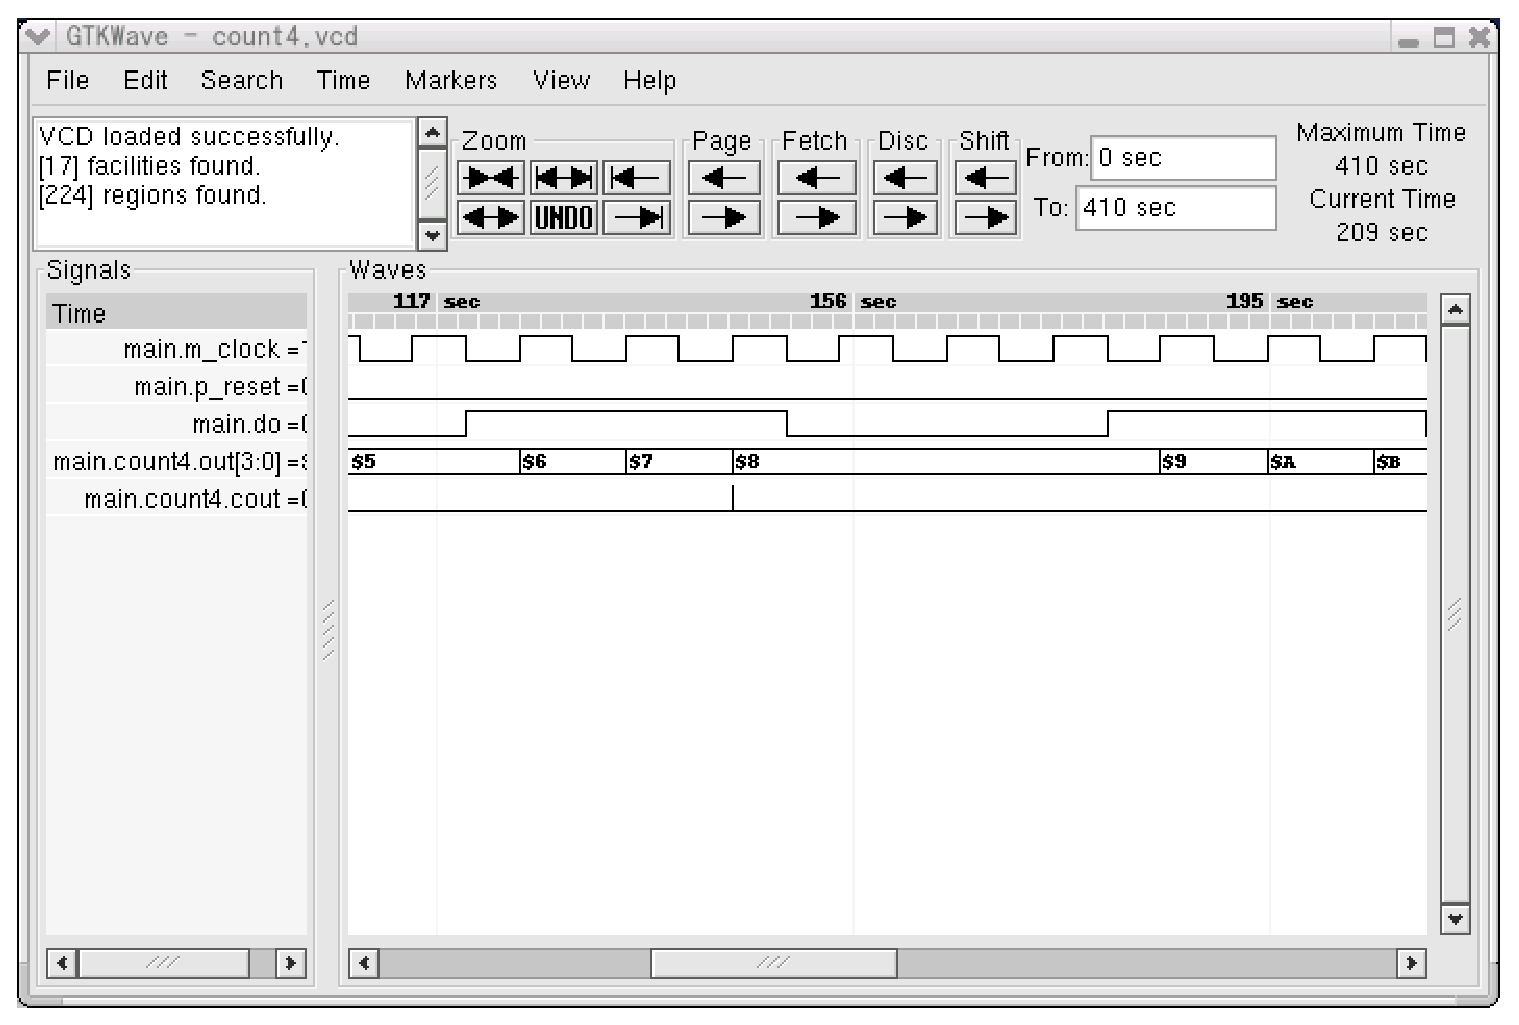
\includegraphics[scale=0.5]{count4_gtkwave.eps}
%\caption{4ビットカウンタをシミュレーションした際の信号波形}
%\label{fig:4ビットカウンタをシミュレーションした際の信号波形}
%\end{center}
%\end{figure}

\end{document}
%%% End of file (report.tex) %%%%%%%%%%%%%%%%%%%%%%%%%%%%%%%%%%%%%%%%%%%%%%
